\documentclass[a4paper]{article}
\usepackage{amsmath,amssymb,amsfonts,amsthm}
\usepackage{multicol}
\usepackage{multirow}
\usepackage{mathtools}
\usepackage{soul}
\usepackage{hyperref}
\hypersetup{
    colorlinks=true,
    linkcolor=blue,
    filecolor=magenta,      
    urlcolor=cyan,
    pdftitle={Overleaf Example},
    pdfpagemode=FullScreen,
    }
\usepackage{color}
\usepackage[table]{xcolor}
\usepackage[T1]{fontenc}
\usepackage{etoolbox}
\usepackage{multicol}
\usepackage{multirow}
\usepackage{fancyhdr}
\usepackage{graphicx}
\usepackage{array}
\usepackage{amsthm}
\usepackage{titlesec}
\usepackage{tikz}
\usetikzlibrary{arrows.meta,calc}
\renewcommand{\baselinestretch}{1.2}

\titleformat*{\section}{\large\bfseries}
\titleformat*{\subsection}{\normalsize\bfseries}

\graphicspath{{C:/Users/teoso/OneDrive/Documents/Tugas Kuliah/Template Math Depart/}}

\newtheorem{theorem}{Theorem}
\newtheorem*{teorema}{Teorema}
\newtheorem*{definisi}{Definisi}
\theoremstyle{definition}
\newtheorem*{bukti}{Bukti}

\newcommand{\Arg}{\text{Arg}}

\begin{document}
\pagenumbering{gobble}
\fancyhead[L]{\textit{Teosofi Hidayah Agung}}
\fancyhead[R]{\textit{5002221132}}
\pagestyle{fancy}
\begin{enumerate}
  \item Tinjau persamaan
\[
u_{xx} + 2u_{xy} + [1 - q(y)]u_{yy} = 0,
\]
dengan
\[
q(y) = 
\begin{cases}
-1, & y < -1, \\
0, & |y| \leq 1, \\
1, & y > 1.
\end{cases}
\]

\begin{enumerate}
  \item Tentukan domain-domain di mana persamaan tersebut bersifat hiperbolik, parabolik, dan eliptik.
  \item Untuk masing-masing dari tiga domain tersebut, tentukan transformasi kanonik dan bentuk kanoniknya.
  \item Gambarlah garis karakteristik untuk kasus hiperbolik.
\end{enumerate}
  \item Tinjau persamaan
  \[
u_{xx} - 6u_{xy} + 9u_{yy} = x y^2.
\]

\begin{enumerate}
  \item Carilah sistem koordinat \( (s, t) \) sehingga persamaan tersebut berbentuk:
  \[
  9v_{tt} = \frac{1}{3}(s - t)t^2.
  \]
  
  \item Carilah solusi umum \( u(x, y) \).
  \item Carilah solusi dari persamaan yang memenuhi kondisi awal:
  \[
  u(x, 0) = \sin x, \quad u_y(x, 0) = \cos x, \quad \text{untuk semua } x \in \mathbb{R}.
  \]
\end{enumerate}

  
\end{enumerate}
\newpage
\begin{center}
\textbf{SOLUSI}
\end{center}
\begin{enumerate}
  \item Diketahui $A= 1$, $B = 2$, $C = 1 - q(y)$
  \begin{enumerate}
    \item 
    \begin{itemize}
      \item Untuk hiperbolik haruslah $B^2 - 4AC > 0$:
      \[
      B^2 - 4AC = 2^2 - 4(1)(1 - q(y)) = 4 - 4 + 4q(y) = 4q(y) > 0 \Rightarrow q(y) > 0.
      \]
      Hal ini terjadi untuk $y > 1$. Jadi domain hiperbolik adalah $D:= \{(x,y) \in \mathbb{R}^2 : y > 1\}$.
      \item Untuk parabolik haruslah $B^2 - 4AC = 0$:
      \[
      B^2 - 4AC = 2^2 - 4(1)(1 - q(y)) = 4 - 4 + 4q(y) = 4q(y) = 0 \Rightarrow q(y) = 0.
      \]
      Hal ini terjadi untuk $|y| \leq 1$. Jadi domain parabolik adalah $D:= \{(x,y) \in \mathbb{R}^2 : |y| \leq 1\}$.
      \item Untuk eliptik haruslah $B^2 - 4AC < 0$:
      \[
      B^2 - 4AC = 2^2 - 4(1)(1 - q(y)) = 4 - 4 + 4q(y) = 4q(y) < 0 \Rightarrow q(y) < 0.
      \]
      Hal ini terjadi untuk $y < -1$. Jadi domain eliptik adalah $D:= \{(x,y) \in \mathbb{R}^2 : y < -1\}$.
    \end{itemize}
    \item Ingat bahwa 
    \begin{itemize}
      \item Hiperbolik terjadi saat $q(y) = 1$ yang artinya persamaan tersebut berbentuk
      \[
      u_{xx} + 2u_{xy} = 0.
      \]
      Dari persamaan kuadratik diperoleh
      \begin{align*}
      \frac{dy}{dx} &= \frac{B + \sqrt{B^2 - 4AC}}{2A} = \frac{2 + \sqrt{4}}{2} = 2, \\
      \frac{dy}{dx} &= \frac{B - \sqrt{B^2 - 4AC}}{2A} = \frac{2 - \sqrt{4}}{2} = 0.
      \end{align*}
      Kemudian didapatkan hasil integrasi
      \begin{align*}
        \xi(x,y) &= y-2x = c_1, \\
        \eta(x,y) &= y = c_2.
      \end{align*}
      Setelah itu, kita dapatkan turunan
      \begin{align*}
        \xi_x &= -2, & \eta_x &= 0, &
        \xi_y &= 1, & \eta_y &= 1, \\
        \xi_{xx} &= 0, & \eta_{xx} &= 0, &
        \xi_{xy} &= 0, & \eta_{xy} &= 0, \\
        \xi_{yy} &= 0, & \eta_{yy} &= 0.
      \end{align*}
      Lebih lanjut, substitusi ke dalam variabel transformasi yaitu
      \begin{align*}
        A^* &= C^* = D^* = E^* = F^* = G^* = 0, \\
        B^* &= -4
      \end{align*}
      Terakhir adalah persamaan kanoniknya yaitu
      \begin{align*}
        A^* w_{\xi\xi} + B^* w_{\xi\eta} + C^* w_{\eta\eta} + D^* w_{\xi} + E^* w_{\eta} + F^* w + G^* &= 0 \\
        -4 w_{\xi\eta} &= 0 \\
        w_{\xi\eta} &= 0.
      \end{align*}
      \item Parabolik terjadi saat $q(y) = 0$ yang artinya persamaan tersebut berbentuk
      \[
      u_{xx} + 2u_{xy} + u_{yy} = 0.
      \]
      Dari persamaan kuadratik diperoleh
      \begin{align*}
        \frac{dy}{dx} &= \frac{B}{2A} = \frac{2}{2} = 1
      \end{align*}
      Kemudian didapatkan hasil integrasi
      \begin{align*}
        \xi(x,y) &= y-x = c_1
      \end{align*}
      Pilih fungsi $\eta(x,y)=x=c_2$ agar solusinya nanti tunggal. Hal ini dapat dicek menggunakan jacobian
      \begin{align*}
        J &= \begin{vmatrix}
          \xi_x & \xi_y \\
          \eta_x & \eta_y
        \end{vmatrix} = 
        \begin{vmatrix}
          -1 & 1 \\
          1 & 0
        \end{vmatrix} = -1\ne 0.
      \end{align*}
      Setelah itu, kita dapatkan turunan
      \begin{align*}
        \xi_x &= -1, & \eta_x &= 1, &
        \xi_y &= 1, & \eta_y &= 0, \\
        \xi_{xx} &= 0, & \eta_{xx} &= 0, &
        \xi_{xy} &= 0, & \eta_{xy} &= 0, \\
        \xi_{yy} &= 0, & \eta_{yy} &= 0.
      \end{align*}
      Lebih lanjut, substitusi ke dalam variabel transformasi yaitu
      \begin{align*}
        A^* &= B^* = D^* = E^* = F^* = G^* = 0, \\
        C^* &= 1.
      \end{align*}
      Terakhir adalah persamaan kanoniknya yaitu
      \begin{align*}
        A^* w_{\xi\xi} + B^* w_{\xi\eta} + C^* w_{\eta\eta} + D^* w_{\xi} + E^* w_{\eta} + F^* w + G^* &= 0 \\
        w_{\eta\eta} &= 0.
      \end{align*}
      \item Eliptik terjadi saat $q(y) = -1$ yang artinya persamaan tersebut berbentuk
      \[
      u_{xx} + 2u_{xy} + 2u_{yy} = 0.
      \]
      Dari persamaan kuadratik diperoleh
      \begin{align*}
        \frac{dy}{dx} &= \frac{B + \sqrt{B^2 - 4AC}}{2A} = \frac{2 + \sqrt{-4}}{2} = 1 + i, \\
        \frac{dy}{dx} &= \frac{B - \sqrt{B^2 - 4AC}}{2A} = \frac{2 - \sqrt{-4}}{2} = 1 - i.
      \end{align*}
      Kemudian didapatkan hasil integrasi
      \begin{align*}
        \alpha &= y - (1+i)x = c_1, \\
        \beta &= y - (1-i)x = c_2.
      \end{align*}
      Diperoleh fungsi $\xi(x,y)$ dan $\eta(x,y)$ adalah
      \begin{align*}
        \xi(x,y) &= \frac{\alpha+\beta}{2} = \frac{[y-(1+i)x] +[y-(1-i)x]}{2} = y-x, \\
        \eta(x,y) &= \frac{\alpha-\beta}{2i} = \frac{[y-(1+i)x] -[y-(1-i)x]}{2i} = x.
      \end{align*}
      Setelah itu, kita dapatkan turunan
      \begin{align*}
        \xi_x &= -1, & \eta_x &= 1, &
        \xi_y &= 1, & \eta_y &= 0, \\
        \xi_{xx} &= 0, & \eta_{xx} &= 0, &
        \xi_{xy} &= 0, & \eta_{xy} &= 0, \\
        \xi_{yy} &= 0, & \eta_{yy} &= 0.
      \end{align*}
      Lebih lanjut, substitusi ke dalam variabel transformasi yaitu
      \begin{align*}
        A^* &= C^* = 1, \\
        B^* &= D^* = E^* = F^* = G^* = 0.
      \end{align*}
      Terakhir adalah persamaan kanoniknya yaitu
      \begin{align*}
        A^* w_{\xi\xi} + B^* w_{\xi\eta} + C^* w_{\eta\eta} + D^* w_{\xi} + E^* w_{\eta} + F^* w + G^* &= 0 \\
        w_{\xi\xi} + w_{\eta\eta} &= 0.
      \end{align*}
    \end{itemize}
    \item Karakteristik untuk kasus hiperbolik adalah garis-garis yang memenuhi persamaan
    \[
    \xi(x,y) = y - 2x, \quad \eta(x,y) = y 
    \]
    untuk $y > 1$. Dengan kata lain, garis-garis tersebut adalah garis-garis yang sejajar dengan garis $y = 2x + c_1$ dan $y = c_2$ untuk $c \in \mathbb{R}$.
    \begin{figure}[h!htb]
      \centering
      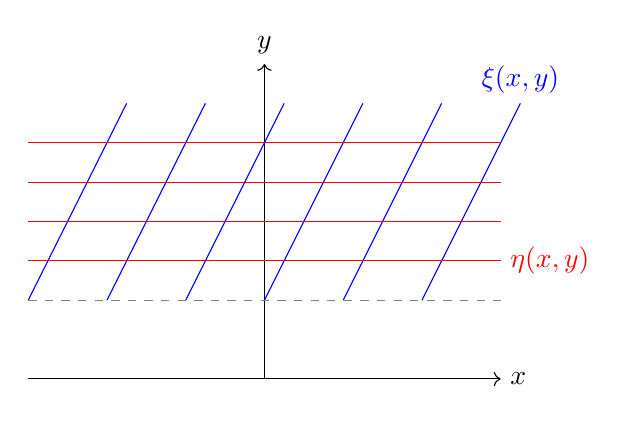
\begin{tikzpicture}
        \draw[->] (-3,0) -- (3,0) node[right] {$x$};
        \draw[->] (0,0) -- (0,4) node[above] {$y$};

        \draw[domain=1:3.5,smooth,variable=\y,blue] plot ({1/2*(\y-1)},{\y}) node[above] {};
        \draw[domain=1:3.5,smooth,variable=\y,blue] plot ({1/2*(\y+1)},{\y}) node[above] {};
        \draw[domain=1:3.5,smooth,variable=\y,blue] plot ({1/2*(\y-3)},{\y}) node[above] {};
        \draw[domain=1:3.5,smooth,variable=\y,blue] plot ({1/2*(\y+3)},{\y}) node[above] {$\xi(x,y)$};
        \draw[domain=1:3.5,smooth,variable=\y,blue] plot ({1/2*(\y-7)},{\y}) node[above] {};
        \draw[domain=1:3.5,smooth,variable=\y,blue] plot ({1/2*(\y-5)},{\y}) node[above] {};

        \draw[domain=-3:3,smooth,variable=\x,red] plot ({\x},{2}) node[right] {};
        \draw[domain=-3:3,smooth,variable=\x,red] plot ({\x},{3}) node[right] {};
        \draw[domain=-3:3,smooth,variable=\x,red] plot ({\x},{1.5}) node[right] {$\eta(x,y)$};
        \draw[domain=-3:3,smooth,variable=\x,red] plot ({\x},{2.5}) node[right] {};

        \draw[dashed,gray] (-3,1) -- (3,1);
      \end{tikzpicture}
    \end{figure}
  \end{enumerate}
  
  \item Persamaan yang diberikan adalah
\[
u_{xx}\;-\;6\,u_{xy}\;+\;9\,u_{yy}\;=\;x\,y^{2}.
\]
  
  \begin{enumerate}
    \item Cari sistem koordinat \((s,t)\) sehingga persamaan menjadi
\[
9\,v_{tt} \;=\;\tfrac{1}{3}\,(s - t)\,t^{2}.
\]
Di sini kita akan melakukan transformasi perubahan variabel dari \((x,y)\) ke \((s,t)\). Karena koefisien bagian diferensial memenuhi
\[
A \;=\; 1,\quad B \;=\;-3,\quad C \;=\;9 
\quad\Longrightarrow\quad
B^{2} - A\,C \;=\;9 - 9 \;=\;0,
\]
maka persamaan ini bersifat parabolik, dan karakteristik tunggalnya adalah
\[
\frac{dy}{dx} \;=\;-3 
\quad\Longrightarrow\quad 
y + 3\,x = c_1
\]
Jadi kita dapat memilih salah satu variabel baru (misalnya \(s\)) sebagai
\[
s \;=\; y \;+\; 3\,x,
\]
dan variabel bebas kedua kita pilih sebagai
\[
t \;=\; x.
\]
Dengan demikian, kita mendefinisikan
\[
\begin{cases}
s \;=\; y + 3\,x,\\
t \;=\; x.
\end{cases}
\quad\Longrightarrow\quad
\begin{cases}
x \;=\; t,\\
y \;=\; s \;-\; 3\,t.
\end{cases}
\]
Sekarang kita tulis \(u(x,y)\) sebagai fungsi \(v(s,t)\):
\[
u(x,y)\;=\;v\bigl(s(x,y),\,t(x,y)\bigr)
\;=\;v\bigl(\,y +3\,x,\;x\bigr).
\]
Langkah selanjutnya adalah menghitung turunan parsial \(u_{xx},\,u_{xy},\,u_{yy}\) dalam bentuk turunan parsial \(v_{ss},\,v_{st},\,v_{tt}\).  

Hitung dulu turunan pertama
   \[
   \begin{aligned}
   u_{x} 
   &= \frac{\partial v}{\partial s}\,\frac{\partial s}{\partial x}
     \;+\;\frac{\partial v}{\partial t}\,\frac{\partial t}{\partial x} 
   \;=\; v_{s}\cdot 3 \;+\; v_{t}\cdot 1 
   \;=\;3\,v_{s} \;+\; v_{t},\\
   u_{y} 
   &= \frac{\partial v}{\partial s}\,\frac{\partial s}{\partial y}
     \;+\;\frac{\partial v}{\partial t}\,\frac{\partial t}{\partial y} 
   \;=\; v_{s}\cdot 1 \;+\; v_{t}\cdot 0 
   \;=\; v_{s}.
   \end{aligned}
   \]

Untuk turunan kedua, didapatkan
   \begin{align*}
      u_{xx} 
     &= \frac{\partial}{\partial x}\bigl(3\,v_{s} + v_{t}\bigr) 
     = 3\,\bigl(v_{ss}\,\tfrac{\partial s}{\partial x} + v_{st}\,\tfrac{\partial t}{\partial x}\bigr)
       \;+\; \bigl(v_{ts}\,\tfrac{\partial s}{\partial x} + v_{tt}\,\tfrac{\partial t}{\partial x}\bigr)\\
     &= 3\,\bigl(v_{ss}\cdot 3 + v_{st}\cdot 1\bigr) \;+\; \bigl(v_{ts}\cdot 3 + v_{tt}\cdot 1\bigr)\\
     &= 9\,v_{ss} \;+\; 3\,v_{st} \;+\; 3\,v_{ts} \;+\; v_{tt}
     \;=\; 9\,v_{ss} \;+\; 6\,v_{st} \;+\; v_{tt}\\
     u_{xy}
     &= 3\,\bigl(v_{ss}\,\tfrac{\partial s}{\partial y} + v_{st}\,\tfrac{\partial t}{\partial y}\bigr)
       \;+\; \bigl(v_{ts}\,\tfrac{\partial s}{\partial y} + v_{tt}\,\tfrac{\partial t}{\partial y}\bigr)\\
     &= 3\,\bigl(v_{ss}\cdot 1 + v_{st}\cdot 0\bigr) \;+\; \bigl(v_{ts}\cdot 1 + v_{tt}\cdot 0\bigr) \\
     &= 3\,v_{ss} \;+\; v_{ts} \\
     &= 3\,v_{ss} \;+\; v_{st}\\
     u_{yy} 
     &= v_{ss}\,\frac{\partial s}{\partial y} + v_{st}\,\frac{\partial t}{\partial y}\\
     &= v_{ss}\cdot 1 + v_{st}\cdot 0 \\
     &= v_{ss}
   \end{align*}

  Subtitusi ke PDP awal
   \[
   \begin{aligned}
   u_{xx} \;-\; 6\,u_{xy} \;+\; 9\,u_{yy}
   &= \bigl(9\,v_{ss} + 6\,v_{st} + v_{tt}\bigr) 
     \;-\; 6\,\bigl(3\,v_{ss} + v_{st}\bigr) 
     \;+\; 9\,\bigl(v_{ss}\bigr) \\[6pt]
   &= 9\,v_{ss} + 6\,v_{st} + v_{tt} 
     \;-\; 18\,v_{ss} - 6\,v_{st} 
     \;+\; 9\,v_{ss} \\[4pt]
   &= \bigl(9 - 18 + 9\bigr)\,v_{ss} 
     \;+\;\bigl(6 - 6\bigr)\,v_{st} 
     \;+\; v_{tt}
   \;=\; v_{tt}.
   \end{aligned}
   \]
   Dengan demikian, di dalam variabel \((s,t)\) kita peroleh
   \[
   u_{xx} - 6\,u_{xy} + 9\,u_{yy} 
   \;=\; v_{tt}.
   \]
   Sisi kanan persamaan awal adalah \( x\,y^{2} \). Karena \(x = t\) dan \(y = s - 3\,t\), maka
   \[
   x\,y^{2} 
   = t \cdot \bigl(s - 3\,t\bigr)^{2}.
   \]
   Jadi PDE transformasi menjadi
   \[
   v_{tt} \;=\; t\,\bigl(s - 3\,t\bigr)^{2}.
   \]
   Jika kita mengalikan kedua ruas dengan 9, diperoleh bentuk yang diinginkan:
   \[
   9\,v_{tt} \;=\; 9\,t\,\bigl(s - 3\,t\bigr)^{2}.
   \]
   karena inilah bentuk kanonik yang sahih dari transformasi \(s=y+3x,\;t=x\).

\item Cari solusi umum \(u(x,y)\)

Karena \(v_{tt} = t\,(s - 3\,t)^{2}\), kita anggap \(s\) sebagai parameter konstan saat mengintegrasi terhadap \(t\). Langkah-langkah integrasinya:
   \[
   \begin{aligned}
   v_{tt} \;=\; t\,\bigl(s - 3\,t\bigr)^{2} 
   &= t\,\bigl(s^{2} - 6\,s\,t + 9\,t^{2}\bigr)
   \;=\; s^{2}\,t \;-\; 6\,s\,t^{2} \;+\; 9\,t^{3}.
   \end{aligned}
   \]
   Integrasikan sekali terhadap \(t\):
   \[
   v_{t}(s,t) 
   = \int \bigl(s^{2}\,t \;-\; 6\,s\,t^{2} \;+\; 9\,t^{3}\bigr)\,dt 
   = \frac{s^{2}\,t^{2}}{2} \;-\; 2\,s\,t^{3} \;+\; \frac{9\,t^{4}}{4} \;+\; A(s),
   \]
   di mana \(A(s)\) adalah “konstanta integrasi” yang boleh bergantung pada \(s\), karena kita hanya mengintegrasi terhadap \(t\).


   \[
   v(s,t) 
   = \int v_{t}(s,t)\;dt 
   = \int \Bigl(\frac{s^{2}\,t^{2}}{2} \;-\; 2\,s\,t^{3} \;+\; \frac{9\,t^{4}}{4} \;+\; A(s)\Bigr)\,dt.
   \]
   Hitung satu per satu:
   - \(\displaystyle \int \frac{s^{2}\,t^{2}}{2}\,dt 
   = \frac{s^{2}}{2} \cdot \frac{t^{3}}{3} 
   = \frac{s^{2}\,t^{3}}{6}.\)
   - \(\displaystyle \int \bigl(-2\,s\,t^{3}\bigr)\,dt 
   = -2\,s \cdot \frac{t^{4}}{4} 
   = -\frac{s\,t^{4}}{2}.\)
   - \(\displaystyle \int \frac{9\,t^{4}}{4}\,dt 
   = \frac{9}{4} \cdot \frac{t^{5}}{5} 
   = \frac{9\,t^{5}}{20}.\)
   - \(\displaystyle \int A(s)\,dt = A(s)\,t + B(s),\)  
     di mana \(B(s)\) adalah konstanta integrasi kedua (boleh bergantung pada \(s\)).

   Dengan demikian:
   \[
   v(s,t) 
   = \frac{s^{2}\,t^{3}}{6} \;-\; \frac{s\,t^{4}}{2} \;+\; \frac{9\,t^{5}}{20} \;+\; A(s)\,t \;+\; B(s).
   \]

   Kita sudah menetapkan
   \[
   s = y + 3\,x,\quad t = x,
   \quad\text{dan}\quad
   u(x,y) = v\bigl(y + 3\,x,\;x\bigr).
   \]
   Jadi solusi umum \(u(x,y)\) adalah:
   \[
   \boxed{
   u(x,y) 
   \;=\; 
   \frac{\bigl(y + 3\,x\bigr)^{2}\,x^{3}}{6}
   \;-\; \frac{\bigl(y + 3\,x\bigr)\,x^{4}}{2}
   \;+\; \frac{9\,x^{5}}{20}
   \;+\; A\bigl(y + 3\,x\bigr)\,x
   \;+\; B\bigl(y + 3\,x\bigr)\,,
   }
   \]
   di mana \(A\) dan \(B\) adalah dua fungsi bebas satu variabel (masing‐masing bergantung hanya pada \(s = y+3x\)).


\item Solusi khusus yang memenuhi kondisi awal
\[
u(x,0) \;=\; \sin x,\qquad u_{y}(x,0) \;=\; \cos x,\quad \forall\,x\in\mathbb{R}.
\]
Kita substitusikan \(y=0\) (oleh karena itu \(s = y + 3x = 3x\) dan \(t = x\)) ke dalam bentuk solusi umum, lalu terapkan kondisi awal untuk menentukan fungsi \(A(s)\) dan \(B(s)\).

   Bila \(y=0\), maka \(s = 3x\) dan \(t = x\). Dari solusi umum:
   \[
   u(x,0)
   = \frac{(3x)^{2}\,x^{3}}{6}
     \;-\;\frac{(3x)\,x^{4}}{2}
     \;+\;\frac{9\,x^{5}}{20}
     \;+\;A(3x)\,x
     \;+\;B(3x).
   \]
   Hitung suku‐suku pangkat \(x\):
   - \(\displaystyle \frac{(3x)^{2}\,x^{3}}{6} 
     = \frac{9\,x^{2}\,x^{3}}{6} 
     = \frac{9\,x^{5}}{6} 
     = \frac{3\,x^{5}}{2}.\)
   - \(\displaystyle -\,\frac{(3x)\,x^{4}}{2} 
     = -\,\frac{3\,x^{5}}{2}.\)
   - \(\displaystyle \frac{9\,x^{5}}{20}\) tetap.

   Jadi
   \[
   \begin{aligned}
   u(x,0)
   &= \Bigl(\tfrac{3\,x^{5}}{2}\;-\;\tfrac{3\,x^{5}}{2} + \tfrac{9\,x^{5}}{20}\Bigr)
     \;+\;A(3x)\,x \;+\; B(3x)\\
   &= \frac{9\,x^{5}}{20} \;+\; A(3x)\,x \;+\; B(3x).
   \end{aligned}
   \]
   Tetapi kita ingin \(u(x,0) = \sin x\). Dengan demikian:
   \[
   \frac{9\,x^{5}}{20} \;+\; A(3x)\,x \;+\; B(3x) \;=\; \sin x,
   \quad \forall\,x.
   \]
   Susun ulang:
   \[
   A(3x)\,x + B(3x) 
   \;=\; \sin x \;-\; \frac{9\,x^{5}}{20}.
   \]
   Definisikan \(s = 3x\). Maka \(x = s/3\). Tuliskan:
   \[
   A(s)\,\bigl(\tfrac{s}{3}\bigr) \;+\; B(s) 
   \;=\; \sin\Bigl(\tfrac{s}{3}\Bigr) \;-\; \frac{9\,\bigl(\tfrac{s}{3}\bigr)^{5}}{20}.
   \]
   Atau
   \[
   \frac{s}{3}\,A(s) \;+\; B(s) 
   = \sin\Bigl(\tfrac{s}{3}\Bigr)
     \;-\; \frac{9}{20}\,\frac{s^{5}}{3^{5}} 
   = \sin\Bigl(\tfrac{s}{3}\Bigr)
     \;-\; \frac{9\,s^{5}}{20 \cdot 243}.
   \]
   Karena \(20 \cdot 243 = 4860\), suku polinomialnya menjadi \(\tfrac{9}{4860}\,s^{5} = \tfrac{s^{5}}{540}\). Jadi secara ringkas:
   \[
   \frac{s}{3}\,A(s) \;+\; B(s) 
   = \sin\!\bigl(\tfrac{s}{3}\bigr) \;-\; \frac{s^{5}}{540}.
   \]
   Kita tidak dapat mengekstrak \(A(s)\) dan \(B(s)\) secara unik dari satu persamaan—karena ada dua fungsi tak tentu. Namun, ingat kita masih punya kondisi awal kedua berupa \(u_{y}(x,0)\). Kita akan memanfaatkan itu untuk mendapatkan persamaan tambahan.


   Dari identitas umum:
   \[
   u(x,y) 
   = v\bigl(s,y\bigr)
   = v\bigl(y + 3x,\;x\bigr),
   \]
   kita dapat menurunkan \(u_{y}\). Tetapi kita sudah menghitung di atas:  
   \[
   u_{y}(x,y) = v_{s}(s,t)\,\frac{\partial s}{\partial y} \;+\; v_{t}(s,t)\,\frac{\partial t}{\partial y} 
   = v_{s}(s,t)\cdot 1 \;+\; v_{t}(s,t)\cdot 0 
   = v_{s}(s,t).
   \]
   Jadi cukup kita hitung
   \[
   v_{s}(s,t) = \frac{\partial}{\partial s}
   \Bigl[\,
   \tfrac{s^{2}\,t^{3}}{6}
   \;-\;\tfrac{s\,t^{4}}{2}
   \;+\;\tfrac{9\,t^{5}}{20}
   \;+\;A(s)\,t
   \;+\;B(s)\Bigr].
   \]
   Turunan terhadap \(s\) (anggap \(t\) konstan) menghasilkan:
   \[
   \begin{aligned}
   v_{s}(s,t) 
   &= \frac{\partial}{\partial s}\Bigl(\tfrac{s^{2}\,t^{3}}{6}\Bigr)
     \;-\;\frac{\partial}{\partial s}\Bigl(\tfrac{s\,t^{4}}{2}\Bigr)
     \;+\; \frac{\partial}{\partial s}\Bigl(\tfrac{9\,t^{5}}{20}\Bigr)
     \;+\; \frac{\partial}{\partial s}\bigl(A(s)\,t\bigr)
     \;+\; \frac{\partial}{\partial s}B(s) \\
   &= \tfrac{2\,s\,t^{3}}{6} 
     \;-\; \tfrac{t^{4}}{2} 
     \;+\; 0 
     \;+\; A'(s)\,t 
     \;+\; B'(s) \\
   &= \frac{s\,t^{3}}{3} 
     \;-\; \frac{t^{4}}{2} 
     \;+\; t\,A'(s) 
     \;+\; B'(s).
   \end{aligned}
   \]
   Sekarang kita terapkan \(y=0\), maka \(s = y+3x = 3x\), \(t=x\). Dengan \(u_{y}(x,0) = v_{s}(3x,\,x)\), kita mesti memenuhi:
  \begin{align*}
  u_{y}(x,0)
  &= v_{s}\bigl(3x,\;x\bigr) \\
  &= \frac{(3x)\,x^{3}}{3} \;-\; \frac{x^{4}}{2} \;+\; x\,A'(3x) \;+\; B'(3x) \\
  &= x^{4} \;-\; \frac{x^{4}}{2} \;+\; x\,A'(3x) \;+\; B'(3x) \\
  &= \frac{x^{4}}{2} \;+\; x\,A'(3x) \;+\; B'(3x).
  \end{align*}
   Karena \(\frac{(3x)\,x^{3}}{3} = x^{4}\cdot\frac{3}{3} = x^{4}\). Jadi detailnya:
   \[
   \frac{(3x)\,x^{3}}{3} = x^{4}, 
   \quad\text{dan}\quad
   x^{4} - \frac{x^{4}}{2} = \frac{x^{4}}{2}.
   \]
   Artinya
   \[
   v_{s}(3x,\,x)
   = \frac{x^{4}}{2} \;+\; x\,A'(3x) \;+\; B'(3x).
   \]
   Kita ingin \(u_{y}(x,0) = \cos x\). Maka
   \[
   \frac{x^{4}}{2} \;+\; x\,A'(3x) \;+\; B'(3x) 
   \;=\; \cos x,
   \quad\forall\,x.
   \]
   Kita gantikan lagi \(s=3x\) → \(x = s/3\). Sehingga
   \[
   \frac{\bigl(\tfrac{s}{3}\bigr)^{4}}{2} 
   \;+\; \bigl(\tfrac{s}{3}\bigr)\,A'(s) 
   \;+\; B'(s) 
   \;=\; \cos\!\bigl(\tfrac{s}{3}\bigr).
   \]
   \[
   \frac{s^{4}}{2\cdot 3^{4}} 
   + \frac{s}{3}\,A'(s) 
   + B'(s) 
   = \cos\!\bigl(\tfrac{s}{3}\bigr).
   \]
   Karena \(3^{4} = 81\), maka \(\tfrac{s^{4}}{2\cdot 81} = \tfrac{s^{4}}{162}\). Jadi
   \[
   \frac{s^{4}}{162} + \frac{s}{3}\,A'(s) + B'(s) 
   = \cos\!\bigl(\tfrac{s}{3}\bigr).
   \]


   Kita sudah punya dua persamaan fungsi untuk \(A\) dan \(B\) (dalam variabel \(s\)):

   - Dari kondisi \(u(x,0)=\sin x\), diperoleh
     \[
     \frac{s}{3}\,A(s) \;+\; B(s) \;=\; \sin\!\bigl(\tfrac{s}{3}\bigr) \;-\; \frac{s^{5}}{540},
     \tag{I}
     \]
     di mana \(s=3x\).

   - Dari kondisi \(u_{y}(x,0)=\cos x\), diperoleh
     \[
     \frac{s^{4}}{162} \;+\; \frac{s}{3}\,A'(s) \;+\; B'(s)
     = \cos\!\bigl(\tfrac{s}{3}\bigr).
     \tag{II}
     \]

      Turunkan di kedua ruas:
      \[
      \frac{d}{ds}\Bigl(\frac{s}{3}\,A(s) + B(s)\Bigr)
      = \frac{d}{ds}\Bigl(\sin\!\bigl(\tfrac{s}{3}\bigr) - \tfrac{s^{5}}{540}\Bigr).
      \]
      - Orbit kiri: 
        \[
        \frac{d}{ds}\Bigl(\tfrac{s}{3}\,A(s)\Bigr) 
        + B'(s)
        = \frac{1}{3}\,A(s) + \frac{s}{3}\,A'(s) + B'(s).
        \]
      - Orbit kanan:
        \[
        \frac{d}{ds}\sin\!\bigl(\tfrac{s}{3}\bigr) 
        - \frac{d}{ds}\Bigl(\tfrac{s^{5}}{540}\Bigr) 
        = \cos\!\bigl(\tfrac{s}{3}\bigr)\cdot\frac{1}{3} 
        \;-\; \frac{5\,s^{4}}{540} 
        = \frac{1}{3}\,\cos\!\bigl(\tfrac{s}{3}\bigr)
          \;-\; \frac{s^{4}}{108}.
        \]
      Maka persamaan turunan (I) menjadi:
      \[
      \frac{1}{3}\,A(s) 
      \;+\; \frac{s}{3}\,A'(s)
      \;+\; B'(s)
      \;=\; \frac{1}{3}\,\cos\!\bigl(\tfrac{s}{3}\bigr)
            \;-\; \frac{s^{4}}{108}.
      \tag{III}
      \]

      Persamaan (II) adalah:
      \[
      \frac{s^{4}}{162} 
      \;+\;\frac{s}{3}\,A'(s) 
      \;+\; B'(s) 
      = \cos\!\bigl(\tfrac{s}{3}\bigr).
      \]
      Kurangkan (III) dari (II) untuk menghilangkan \(\tfrac{s}{3}A'(s) + B'(s)\). Kita lakukan
      \[
      \bigl[\text{(II)}\bigr] \;-\; \bigl[\text{(III)}\bigr]:
      \]
      \[
      \Bigl(\tfrac{s^{4}}{162} + \tfrac{s}{3}A'(s) + B'(s)\Bigr)
      \;-\; \Bigl(\tfrac{1}{3}A(s) + \tfrac{s}{3}A'(s) + B'(s)\Bigr)
      = \cos\!\bigl(\tfrac{s}{3}\bigr)
        \;-\;\Bigl[\tfrac{1}{3}\cos\!\bigl(\tfrac{s}{3}\bigr) - \tfrac{s^{4}}{108}\Bigr].
      \]
      Di ruas kiri, \(\tfrac{s}{3}A'(s) + B'(s)\) saling batal:
      \[
      \frac{s^{4}}{162} \;-\; \frac{1}{3}\,A(s)
      \;=\; \cos\!\bigl(\tfrac{s}{3}\bigr) 
         \;-\; \frac{1}{3}\,\cos\!\bigl(\tfrac{s}{3}\bigr) 
         \;+\; \frac{s^{4}}{108}.
      \]
      \[
      \frac{s^{4}}{162} \;-\; \frac{1}{3}A(s)
      = \frac{2}{3}\,\cos\!\bigl(\tfrac{s}{3}\bigr)
        \;+\; \frac{s^{4}}{108}.
      \]
      Gabungkan suku \(s^{4}\):
      \[
      \frac{s^{4}}{162} \;-\; \frac{s^{4}}{108}
      = \frac{1}{3}\,A(s) 
      \;+\; \frac{2}{3}\,\cos\!\bigl(\tfrac{s}{3}\bigr).
      \]
      Karena \(\tfrac{1}{162} - \tfrac{1}{108} = \tfrac{1}{162} - \tfrac{1.5}{162} = -\,\tfrac{0.5}{162} = -\,\tfrac{1}{324},\) maka
      \[
      -\,\frac{s^{4}}{324}
      = \frac{1}{3}\,A(s) \;+\; \frac{2}{3}\,\cos\!\bigl(\tfrac{s}{3}\bigr).
      \]
      Kalikan kedua ruas dengan 3:
      \[
      -\,\frac{s^{4}}{108}
      = A(s) \;+\; 2\,\cos\!\bigl(\tfrac{s}{3}\bigr).
      \]
      Jadi kita peroleh
      \[
      \boxed{\,A(s) \;=\; -\,\frac{s^{4}}{108} \;-\; 2\,\cos\!\bigl(\tfrac{s}{3}\bigr)\,.}
      \tag{IV}
      \]

      Persamaan (I) adalah:
      \[
      \frac{s}{3}\,A(s) \;+\; B(s)
      = \sin\!\bigl(\tfrac{s}{3}\bigr) \;-\; \frac{s^{5}}{540}.
      \]
      Gantikan \(A(s) = -\tfrac{s^{4}}{108} - 2\cos\bigl(\tfrac{s}{3}\bigr)\):
      \[
      \frac{s}{3}\,\Bigl(-\,\tfrac{s^{4}}{108} \;-\; 2\,\cos\!\bigl(\tfrac{s}{3}\bigr)\Bigr) \;+\; B(s)
      = \sin\!\bigl(\tfrac{s}{3}\bigr) \;-\; \frac{s^{5}}{540}.
      \]
      Hitung \(\displaystyle \frac{s}{3}\cdot\bigl(-\tfrac{s^{4}}{108}\bigr) = -\,\frac{s^{5}}{324}\), dan \(\displaystyle \frac{s}{3}\cdot\bigl(-2\cos(\tfrac{s}{3})\bigr) = -\,\tfrac{2\,s}{3}\,\cos\!\bigl(\tfrac{s}{3}\bigr)\). Jadi:
      \[
      -\,\frac{s^{5}}{324} 
      \;-\; \frac{2\,s}{3}\,\cos\!\bigl(\tfrac{s}{3}\bigr)
      \;+\; B(s)
      = \sin\!\bigl(\tfrac{s}{3}\bigr)
        \;-\; \frac{s^{5}}{540}.
      \]
      Pindahkan semua suku ke satu sisi untuk mengekspresikan \(B(s)\):
      \[
      B(s) 
      = \sin\!\bigl(\tfrac{s}{3}\bigr)
        \;-\; \frac{s^{5}}{540}
        \;+\; \frac{s^{5}}{324}
        \;+\; \frac{2\,s}{3}\,\cos\!\bigl(\tfrac{s}{3}\bigr).
      \]
      Gabungkan \(\displaystyle -\tfrac{s^{5}}{540} + \tfrac{s^{5}}{324}\). Perhatikan:
      \[
      \tfrac{1}{324} - \tfrac{1}{540}
      = \frac{5 - 3}{1620} 
      = \frac{2}{1620} 
      = \frac{1}{810}.
      \]
      Jadi
      \[
      -\,\frac{s^{5}}{540} \;+\; \frac{s^{5}}{324}
      = \frac{s^{5}}{810}.
      \]
      Maka
      \[
      \boxed{\,B(s) 
      = \sin\!\bigl(\tfrac{s}{3}\bigr)
        \;+\; \frac{s^{5}}{810}
        \;+\; \frac{2\,s}{3}\,\cos\!\bigl(\tfrac{s}{3}\bigr)\,.}
      \tag{V}
      \]

   Dengan demikian, kita telah menemukan ekspresi eksplisit untuk \(A(s)\) dan \(B(s)\). Ringkasnya:
   \[
   \begin{cases}
   A(s) = -\,\frac{s^{4}}{108} \;-\; 2\,\cos\!\bigl(\tfrac{s}{3}\bigr),\\
   B(s) = \sin\!\bigl(\tfrac{s}{3}\bigr)
        \;+\; \frac{s^{5}}{810}
        \;+\; \frac{2\,s}{3}\,\cos\!\bigl(\tfrac{s}{3}\bigr).
   \end{cases}
   \]
   Ingat kembali bahwa \(s = y + 3\,x\).  

   Perhatikan bahwa solusi umum:
   \[
   u(x,y)
   = \frac{(y + 3x)^{2}\,x^{3}}{6}
     \;-\; \frac{(y + 3x)\,x^{4}}{2}
     \;+\; \frac{9\,x^{5}}{20}
     \;+\; A\bigl(y+3x\bigr)\,x
     \;+\; B\bigl(y+3x\bigr).
   \]
   Sekarang masukkan \(A\) dan \(B\) sesuai (IV) dan (V). Ingat \(s = y+3x\). Maka
   \[
   \boxed{
   \begin{aligned}
   u(x,y) \;=\; {}& \frac{(y + 3x)^{2}\,x^{3}}{6}
     \;-\; \frac{(y + 3x)\,x^{4}}{2}
     \;+\; \frac{9\,x^{5}}{20}
     \\[6pt]
   &\quad -\,\Bigl(\tfrac{(y+3x)^{4}}{108} + 2\,\cos\!\bigl(\tfrac{y+3x}{3}\bigr)\Bigr)\,x
     \\[6pt]
   &\quad +\,\Bigl[
     \sin\!\bigl(\tfrac{y+3x}{3}\bigr)
     \;+\; \frac{(y+3x)^{5}}{810}
     \;+\; \frac{2\,(y+3x)}{3}\,\cos\!\bigl(\tfrac{y+3x}{3}\bigr)
     \Bigr].
   \end{aligned}
   }
   \]
  \end{enumerate}





\end{enumerate}
\end{document}